\RequirePackage[l2tabu, orthodox]{nag}
\documentclass[11pt, oneside]{article}
\usepackage{geometry}
\geometry{letterpaper}
\usepackage{graphicx}

\usepackage{amssymb}
\usepackage{amsmath}

\usepackage{minted}
\usepackage{hyperref}

\usepackage{color}

\usepackage{graphicx}

\usepackage[english]{babel}
\usepackage[utf8]{inputenc}
\usepackage[T1]{fontenc}
\usepackage{lmodern}

\usepackage{microtype}

\allowdisplaybreaks

\newcommand{\blue}[1]{\textcolor{blue}{#1}}
\newcommand{\red}[1]{\textcolor{red}{#1}}
\newcommand{\green}[1]{\textcolor{green}{#1}}
\newcommand{\pe}[1]{\green{PE: #1}}

\newenvironment{polynomial}
  {\par\vspace{\abovedisplayskip}%
   \setlength{\leftskip}{\parindent}%
   \setlength{\rightskip}{\leftskip}%
   \medmuskip=4mu plus 2mu minus 2mu
   \binoppenalty=0
   \noindent$\displaystyle}
  {$\par\vspace{\belowdisplayskip}}



\newcommand{\ans}[1]{\blue{
\begin{polynomial}
#1
\end{polynomial}
}}


\newcommand{\vect}[1]{\vec{\lowercase{#1}}}

\title{Homework \#4}
\author{
Haylee Crane \\
Paul English
}

\begin{document}
\maketitle

\begin{enumerate}

\item \textbf{(Iterative Solution of Linear Systems.)} Consider the $n \times n$
linear system $Ax=b$ and recall the three iterative techniques we
discussed in class:

\textbf{Gauss-Jacobi:}
\[
x_i^{[k+1]} = \frac{1}{a_{ii}} \left( b_i - \sum_{j=1}^{i-1} a_{ij}
x_j^{[k]} - \sum_{j=i+1}^n a_{ij} x_j^{[k]} \right)
\]

\textbf{Gauss-Seidel:}
\[
x_i^{[k+1]} = \frac{1}{a_{ii}} \left(
b_i - \sum_{j=1}^{i-1} a_{ij} x_j^{[k]} - \sum_{j=i+1}^n a_{ij} x_j^{[k+1]}
\right)
\]

\textbf{Successive Overrelaxation:}
\[
x_i^{[k+1]} =
(1 - w)x_i^{[k]} + \frac{w}{a_{ii}}
\left(
b_i - \sum_{j=1}^{i-1} a_{ij} x_j^{[k]} - \sum_{j=i+1}^n a_{ij} x_j^{[k+1]}
\right)
\]

As we discussed in class, think of $A$ as being split as
\[
A = L + D + U
\]
where $L$ contains the entries of $A$ below the diagonal, $U$ contains
the entries above the diagonal, and $D$ contains the entries on the
diagonal. For example,
\[
A
= \left[\begin{matrix} 1 & 2 \\ 3 & 4 \end{matrix} \right]
= L + D + U
= \left[\begin{matrix} 0 & 0 \\ 3 & 0 \end{matrix} \right]
= \left[\begin{matrix} 1 & 0 \\ 0 & 4 \end{matrix} \right]
= \left[\begin{matrix} 0 & 2 \\ 0 & 0 \end{matrix} \right]
\]

Write the above three iterations as
\[
x^{[k+1]} = T_x^{[k]} + c
\]
and for each of the three methods give $T$ in terms of $L$, $D$, and
$U$, and $c$ in terms of $L$, $D$, $U$ and $b$.

Note: in class we derived the correct expressions for the Gauss-Jacobi
method. There was a mistake in the in-class discussion of the
Gauss-Seidel method, and I left the SOR method as an exercise.

{\color{blue}

\textbf{Gauss-Jacobi:}

\begin{align*}
x_i^{[k+1]} &= \frac{1}{a_{ii}} \left( b_i - \sum_{j=1}^{i-1} a_{ij} x_j^{[k]} - \sum_{j=i+1}^n a_{ij} x_j^{[k]} \right) \\
x^{[k+1] }&= D^{-1} \left( b - L x^{[k]} - U x^{[k]} \right) \\
&= D^{-1} \left( b - \left(L + U\right) x^{[k]} \right) \\
&= -D^{-1} \left( L + U \right) x^{[k]} + D^{-1} b \\
\end{align*}
\begin{align*}
\Rightarrow T &= -D^{-1} \left( L + U \right) \\
c &= D^{-1} b
\end{align*}

\textbf{Gauss-Seidel:}
\begin{align*}
x_i^{[k+1]} &= \frac{1}{a_{ii}} \left(b_i - \sum_{j=1}^{i-1} a_{ij}
x_j^{[k]} - \sum_{j=i+1}^n a_{ij} x_j^{[k+1]} \right) \\
x^{[k+1] }&= D^{-1} \left( b - L x^{[k]} - U x^{[k+1]} \right) \\
x^{[k+1] }&= D^{-1} b - D^{-1} L x^{[k]} - D^{-1} U x^{[k+1]}  \\
(I + D^{-1} U) x^{[k+1]} &= D^{-1} b - D^{-1} L x^{[k]} \\
x^{[k+1]} &= - (I + D^{-1} U)^{-1} D^{-1} L x^{[k]} + (I + D^{-1} U)^{-1} D^{-1} b  \\
\end{align*}
\begin{align*}
\Rightarrow
T &= - (I + D^{-1} U)^{-1} D^{-1} L \\
c &= (I + D^{-1} U)^{-1} D^{-1} b
\end{align*}

\textbf{Successive Overrelaxation:}

\begin{align*}
x_i^{[k+1]} &= (1 - w)x_i^{[k]} + \frac{w}{a_{ii}} \left(b_i
- \sum_{j=1}^{i-1} a_{ij} x_j^{[k]} - \sum_{j=i+1}^n a_{ij}
x_j^{[k+1]} \right) \\
x^{[k+1]} &= \left(1-\omega\right) x^{[k]} + \omega D^{-1} \left( b -
L x^{[k]} - U x^{[k+1]}\right) \\
&= \left( 1 - \omega \right) x^{[k]} + \omega D^{-1} b - \omega
D^{-1} L x^{[k]} - \omega D^{-1} U x^{[k+1]} \\
\left( I + \omega D^{-1} U \right) x^{[k+1]} &= \left( \left( 1
- \omega \right)  - \omega D^{-1} L \right)  x^{[k]} + \omega D^{-1} b \\
x^{[k+1]} &= \left( I + \omega D^{-1} U \right)^{-1} \left( \left( 1
- \omega \right) - \omega D^{-1} L \right) x^{[k]} + \left( I
+ \omega D^{-1} U \right) \omega D^{-1} b
\end{align*}
\begin{align*}
\Rightarrow
T &= \left( I + \omega D^{-1} U \right)^{-1} \left( \left( 1
- \omega \right) - \omega D^{-1} L \right)\\
c &= \left( I + \omega D^{-1} U \right) \omega D^{-1}
\end{align*}

}

\item \textbf{(Positive Definite Matrices.)}  A \textit{principal submatrix}
$A_I$ of  an $n \times n$ matrix $A$ is obtained by picking a set $I
\subset \{1,2,\dots,n\}$ and crossing out all rows and columns whose
indices are not in $I$. For example, if \[
A = \left[
  \begin{matrix}
    a_{11} & a_{12} & a_{13} & a_{14} \\
    a_{21} & a_{22} & a_{23} & a_{24}\\
    a_{31} & a_{32} & a_{33} & a_{34}\\
    a_{41} & a_{42} & a_{43} & a_{44}
\end{matrix}
\right]
\]
then the principal submatrix corresponding to the set $\{2,4\}$ is \[
A_{\{2,4\}} = \left[
  \begin{matrix}
  a_{22} & a_{24} \\
  a_{42} & a_{44} \\
  \end{matrix}
\right]
\]
Show that every principal submatrix of a positive definite matrix is
positive definite.

{\color{blue}

% http://www.hss.caltech.edu/~kcb/Notes/QuadraticForms.pdf
% page 4

}

\item \textbf{(The $UL$ factorization.)} Show how to compute the
factorization $A = UL$ where $U$ is upper triangular with $1$s along
the diagonal and $L$ is lower triangular. Show how this relates to a
way of solving $Ax=b$ by transforming the system into an equivalent
system with a lower triangular matrix. (In other words, show that what
we did for the $LU$ factorization also works for a $UL$
factorization.) Note: For the purposes of this exercise you may assume
that no pivoting is required. This is of course unrealistic but
pivoting would only distract from the point of this exercise (which is
that conceptually there is no difference between an $LU$ and a $UL$
factorization).

{\color{blue}



}

\item \textbf{(Spectral Radius.)} We saw that the spectral radius of a
(square) matrix $A$ never exceeds an induced matrix norm of $||A||$.
It can be shown that for any particular matrix $A$ one can find a
vector norm such that the induced matrix norm of $A$ is arbitrarily
close to the spectral radius of $A$. Does the spectral radius itself
define a norm? Why, or why not?

{\color{blue}
\begin{aligned}
Consider\,  0&=\begin{pmatrix}
0 & 0\\ 
0 & 0
\end{pmatrix}
and\, A=
\begin{pmatrix}
0 & 0\\ 
0 & 0
\end{pmatrix}\\
Clearly, A&\neq 0\\
$The eigenvalues of 0 and A are \{0,0\}\\
\Rightarrow \rho(A)=\rho(0)= max\{0,0\}=0\\
Norm\,requires \left \| A \right \|\rightarrow A=0\\
and\, \rho(A)=0\, b,but A\neq0\\
Hence,\, \rho \,is\, \underline{not}\,a \,matrix \,norm

\end{aligned}

}

\item \textbf{(Inequalities are sharp.)} Explain the meaning of \[
\frac{1} {\|A\| \|A^{-1}\|}
\frac{\|r\|} {\|b\|}
\le
\frac{\|e\|}{\|x\|}
\le
\|A\| \|A^{-1}\|
\frac{\|r\|} {\|b\|}
\] and show how we derived these inequalities in class.

\begin{itemize}
\item For a general matrix $A$, and $\| \cdot \| = \| \cdot \|_2$,
  show that there are non-trivial examples (i.e. $x \ne 0 \ne e$)
  where the right hand inequality is satisfied with equality in (3).
  Do the same for the left hand inequality in (3).
\item Repeat part a. for $\| \cdot \| = \| \cdot \|_\infty$.
\end{itemize}

{\color{blue}

$\frac{\| e \|}{\| x \|}$ is the relative error of our linear system,
which may not be computable.
$\frac{\| r \|}{\| b \|}$ is a computable value that we can combine
with the condition number $\| A \| \| A^{-1} \|$ to estimate what the
relative error of our system is.

We say that our system is ill-conditioned if it has a large value for
the condition number, which would mean that the above inequality
doesn't confine the relative error very well. It's well-conditioned
system if the condition number is low, and we can see that the
inequality will give us a narrow bounds and a better estimation of the
relative error.

To derive these equations we have the following equations from our
linear system,

\begin{align*}
Ax &= b \\
A^{-1}b &= x \\
Ae &= r \\
A^{-1}r &= e
\end{align*}

Where $e$ is our error $x - \hat{x}$ therefore $r$ is a relation of
the error and our system.

Using the Cauchy-Schwarz inequality we know that the norms of the
above equations follow these inequalities,
\begin{align*}
\| b \| &\le \| A \| \| x \| \\
\| x \| &\le \| A^{-1} \| \| b \| \\
\| r \| &\le \| A \| \| e \| \\
\| e \| &\le \| A^{-1} \| \| r \| \\
\end{align*}

We can divide the first inequality from the fourth and the second from
the third (we take the reciprocal reversing the inequality and multiply) to arrive at
\begin{align*}
\frac{\| e \|}{\| A \| \|x \|} &\le \frac{\| A^{-1} \| \| r \|}{\| b \|} \\
\frac{\| r \|}{\| A^{-1} \| \| b \|} &\le \frac{\| A \| \| e \|}{\| x \|} \\
\end{align*}

Now with the new set of inequalities we multiply the first by $\|
A \|$ and the second by $\frac{1}{\| A\|}$ to get to the original inequality,
\begin{align*}
\frac{1} {\|A\| \|A^{-1}\|} \frac{\|r\|} {\|b\|}
\le
\frac{\|A\|\|e\|}{\| A\|\|x\|}
\le
\|A\| \|A^{-1}\| \frac{\|r\|} {\|b\|} \\
\Rightarrow \frac{1} {\|A\| \|A^{-1}\|} \frac{\|r\|} {\|b\|}
\le
\frac{\|e\|}{\|x\|}
\le
\|A\| \|A^{-1}\| \frac{\|r\|} {\|b\|}
\end{align*}

For $\| \cdot \| = \| \cdot \|_2$ we have that
$\| A \| = \max_{Ax = \lambda x} \{\lambda\} = \sqrt{\lambda_1}$ or
the square root of the largest eigenvalue, thus
the norm of $A^{-1}$ will be one over the square root of the smallest eigenvalue
$\| A^{-1} \| = \frac{1}{\min_{Ax = \lambda x} \{\lambda\}}
= \sqrt{\frac{1}{\lambda_n}}$ since the eigenvalues of an
inverted matrix are reciprocals. Now our condition number is
$ \|A\| \|A^{-1}\| = \sqrt{\frac{\lambda_1}{\lambda_n}}$, and our
relative error is bounded by,

\begin{align*}
\sqrt{\frac{\lambda_n}{\lambda_1}}
 \frac{\|r\|} {\|b\|}
\le
\frac{\|e\|}{\|x\|}
\le
\sqrt{\frac{\lambda_1}{\lambda_n}}
 \frac{\|r\|} {\|b\|}
\end{align*}

Here inequality is achieved when $\lambda_1 = \lambda_n$. We can find
this case trivially with the identity matrix, i.e.
$A = \begin{bmatrix} 1 & 0 \\ 0 & 1 \end{bmatrix}$.

With $\| \cdot \| = \| \cdot \|_{\infty}$ our matrix norm is
$\| A \| = \max\{ \|a_{ij}\| \} = a_{\max} $ and
$\| A^{-1} \| = \frac{1}{ \min\{\|a_{ij}\|\} } = \frac{1}{a_{\min}}$. This means that our
condition number is
$ \|A\| \|A^{-1}\| = \frac{a_{\max}}{a_{\min}} $, and our inequality will
have the case of equality when $a_{\max} = a_{\min}$. An example of this
is $A = \begin{bmatrix}1 & 0 \\ 0 & -1\end{bmatrix}$.

}

\item \textbf{(Backward Error Analysis.)} This problem explores the effects
of a perturbation in the coefficient matrix (rather than the right
hand side) of the linear system \[Ax=b\] Suppose we solve instead of
(4) the system \[(A - E)(x - e) = b\] where $E$ is a perturpation of
$A$ that causes an error $e$ in the solution $x$. Show that \[
\frac{\|e\|}{\| x - e \|} \le \|A\| \|A^{-1}\| \frac{\| E \|}{\| A \|}
\]

{\color{blue}


}

\item \textbf{(First Order Systems.)} Write the second order initial value
problem
\begin{align}
y^{\prime\prime} &= xy^2 \\
y(0) &= 1 \\
y^\prime(0) &= 2
\end{align}
as an autonomous first order system
\begin{align}
  y^\prime &= f(y)\\
y(a) &= y_0.
\end{align}
(In other words, specify $y$, $f$, $a$, and $y_0$ such that the two
problems are equivalent. Of course, $y$ will have different meanings
for the two problems.)


{\color{blue}
\begin{align*}

y'&=xy^2\\
y(0)&=1\\
y'(0)&=2\\
Let\, z&=y' \, and \, z(0)=2\\
\Rightarrow z'&=xy^2, y(0)=1, z(0)=2\\

\frac{\partial y}{\partial x}&=z, y(0)=1\\
\frac{\partial z}{\partial x}&=xy^2, z(0)=2\\
\Rightarrow Define\, x&=x(t)\, s.t.\frac{\partial x}{\partial t}=1\\
and\,x(0)&=0\\
\Rightarrow \frac{\partial y}{\partial x}&=\frac{\partial y}{\partial x}\frac{\partial x}{\partial t}=z\\
\frac{\partial z}{\partial t}&=\frac{\partial z}{\partial x}\frac{\partial x}{\partial t}=x(t)y^2(t)\\
\Rightarrow \frac{\partial x}{\partial t}&=1, x(0)=0\\
\frac{\partial y}{\partial t}&=z(t), y(x(0))=1\\
\frac{\partial z}{\partial t}&=x(t)y^2(t), z(x(0))=2\\

v&=\begin{bmatrix}
x(t)\\ 
y(t)\\ 
z(t)
\end{bmatrix}, 

f(v)=\begin{bmatrix}
v\\ 
ve_3\\ 
(ve_1)(ve_2)^2
\end{bmatrix}\\

Where \, e_1, e_2, e_3\, are\, the\, &basis\, vectors\,
\begin{bmatrix}
1\\ 
0\\ 
0
\end{bmatrix},
\begin{bmatrix}
0\\ 
1\\ 
0
\end{bmatrix}, 
\begin{bmatrix}
0\\ 
0\\ 
1
\end{bmatrix}
respectively\\

\frac{\partial v}{\partial t}=f(v), v(0)=\begin{bmatrix}
0\\ 
1\\ 
2
\end{bmatrix}

\end{align}


}

\item \textbf{(Improper Integrals.)} Let \[
I = \int_{-1}^1 \frac{\ln (x^2 + 1 )}{\sqrt{1 - x^2}} dx = 2 \pi \ln
\left[ \frac{1 + \sqrt{2}}{2} \right].
\]
This integral is improper because the integrand approaches infinity as
$x$ approaches $\pm 1$. Attempt to approximate this integral by using
Simpson's Rule (or any other Newton-Cotes formula) on the interval
$[-1 + \epsilon, 1 - \epsilon]$ for small $\epsilon > 0$. Describe the
results of your efforts. Then, for $n = 4, 5, 6, 7, 8$, use the
Gaussian Quadrature formula \[
\int_{-1}^1 \frac{f(x)}{\sqrt{1 - x^2}} dx = \frac{\pi}{n}
\sum_{i=1}^n f\left( \cos \left( \frac{(2i - 1) \pi}{2n} \right) \right)
\] which we discussed in class. Compute the error and discuss your results.

{\color{blue}

\begin{minted}[mathescape,
               linenos,
               numbersep=5pt,
               gobble=0,
               frame=lines,
               framesep=2mm]{clojure}
(def I (* 2 Math/PI
           (Math/log (/ (+ 1 (Math/sqrt 2))
                        2))))

(defn gaussian-quadrature [f n]
  (* (/ Math/PI n)
     (->> (range n)
          (map inc)
          (map #(f (Math/cos (/ (* (- (* 2 %) 1)
                                   Math/PI)
                                (* 2 n)))))
          (apply +))))

(def n (range 4 9))

(def results (map #(gaussian-quadrature (fn [x]
                                          (Math/log (+ (Math/pow x 2) 1)))
                                        %)
                  n))
;; => (1.1840219784143866
;;     1.1824745448480443
;;     1.182688104009816
;;     1.1826574630224815
;;     1.1826619812548276)

(def error (->> results
                (map #(Math/abs (- I %)))
                (zipmap [4 5 6 7 8])))
;; => {4 0.0013605869242299118,
;;     5 1.8684664211243707E-4,
;;     6 2.6712519659355394E-5,
;;     7 3.92846767516275E-6,
;;     8 5.897646708774573E-7}
\end{minted}

\begin{figure}[H]
\centering
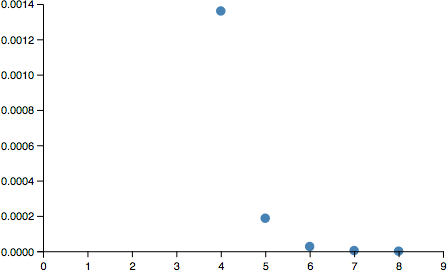
\includegraphics[scale=0.65]{improper-integrals-error.png}
\caption{Error for $n=4,5,6,7,8$.}
\end{figure}

We can see that our error decreases for larger values of $n$ and
approaches $0$ quickly. Even for $n=4$ it's accurate.
}

\item \textbf{(Numerical Comparison.)} For Euler's Method, the Trapezoidal
Rule, Simpson's Rule, and the standard $4$-th order Runge-Kutta
Method solve the initial value problem
\begin{aligned}
y^\prime &= y \\
y(0) = 1\\
x \in [0,1]
\end{aligned}
with step-sizes $h = 2^{-s}$ where $s = 3,4,\dots,15$. Plot the error
at the right end-point, i.e. $y(1) - y_n$ (where $n = 1/h$), against
$h$. You may wish to superimpose the plots. If you like use
appropriate logarithmic graph paper. Comment on your results. (For
Simpson's rule use the exact starting value $y_1 = y(h)$.) Send me
your program by e-mail.

The ``standard'' Runge-Kutta method is:
\[
y_{n+1} = y_n + \frac{h}{6} (K_1 + 2K_2 + 2K_3 + K_4)
\]
where
\begin{aligned}
K_1 &= f(x_n, y_n) \\
K_2 &= f \left(x_n + \frac{h}{2}, y_n + \frac{h}{2} K_1 \right)
K_3 &= f \left(x_n + \frac{h}{2}, y_n + \frac{h}{2} K_2 \right)
K_4 &= f \left(x_n + h, y_n + h K_3 \right)
\end{aligned}

{\color{blue}

\begin{enumerate}
\item \textbf{Euler's Method}
\begin{aligned}
  y_{n+1} - y_n = h f_n
\end{aligned}

\item \textbf{Trapezoidal Rule}
\begin{aligned}
  y_{n+1}- y_n = \frac{h}{2} (f_{n+1} + f_n)
\end{aligned}

\item \textbf{Simpons's Rule}
\begin{aligned}
 _{n+1} - y_n
  y_{n+1}- y_n = \frac{h}{2} (f_{n+1} + f_n)
\end{aligned}Successive Overrelaxation:

}


\end{enumerate}

\end{document}
